\documentclass[aspectratio=169]{beamer}
\usetheme{Copenhagen}
\usecolortheme{beaver}

\setbeamertemplate{navigation symbols}{}

\input{packages.tex}
\pgfplotsset{width=10cm,compat=1.9}

\onehalfspacing
\setlength{\parindent}{3em}
\usetikzlibrary{positioning}

\hypersetup{
    colorlinks=true,
    linkcolor=orange,
    filecolor=magenta,      
    urlcolor=red,
    pdftitle={Course work},
    }

\urlstyle{same}


\definecolor{mGray}{rgb}{0.5,0.5,0.5}
\definecolor{mPurple}{rgb}{0.58,0,0.82}
\definecolor{mGreen}{rgb}{0.5,0.82,0.3}
\definecolor{backgroundColour}{rgb}{0.95,0.95,0.92}


\graphicspath{ {C:/Users/nickk/course_work/imgs/} }

\lstdefinestyle{CStyle}{
    backgroundcolor=\color{backgroundColour},   
    commentstyle=\color{mGreen},
    keywordstyle=\color{magenta},
    numberstyle=\tiny\color{mGray},
    stringstyle=\color{mPurple},
    basicstyle=\footnotesize,
    breakatwhitespace=false,         
    breaklines=true,                 
    captionpos=b,                    
    keepspaces=true,                 
    numbers=left,                    
    numbersep=5pt,                  
    showspaces=false,                
    showstringspaces=false,
    showtabs=false,                  
    tabsize=2,
    language=C
}

\title{Моделювання розвитку епiдемiї
з використанням чисельних методiв}

\author{Коломієць Микола}

\date{Червень 2023}

\begin{document}
    \maketitle
    \begin{frame}{SIR Модель}
        \centering
        \only<1>{
        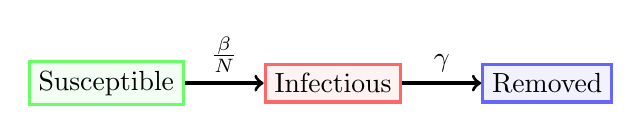
\begin{tikzpicture}
            \node
            [style={rectangle, draw=green!60, fill=green!5, very thick}]
            (Susceptible){Susceptible}; 
            \node
            [style={rectangle, draw=red!60, fill=red!5, very thick}]
            (Infectious)[right=of Susceptible]{Infectious};
            \node
            [style={rectangle, draw=blue!60, fill=blue!5, very thick}]
            (Removed)[right=of Infectious]{Removed};
            \draw[->, style={very thick}] (Susceptible.east)
            to node[above] {$ \frac{\beta}{N} $} (Infectious.west);
            \draw[->, style={very thick}] (Infectious.east)
            to node[above] {$  \gamma $} (Removed.west);
        \end{tikzpicture}}

        
        \begin{block}<2>{Рівняння}
            \begin{equation*}
                \begin{cases}
                    \frac{dS}{dt} = - \frac{\beta}{N}SI          \\
                    \frac{dI}{dt} = \frac{\beta}{N}SI - \gamma I \\
                    \frac{dR}{dt} = \gamma I
                \end{cases}
            \end{equation*}
        \end{block}

    \end{frame}
\end{document}


